\chapterimage{./Pictures/recurrence_equations.png}
\chapter{Ecuaciones de recurrencia}

\section{Introducción}
En el análisis de las ecuaciones de recurrencia tenemos desarrollos de expresiones matemáticas de recurrencia mediante métodos de resolución.
\\~
Cuando divido el problema y cada problema viene con la mitad de los datos, cada nivel tendra un árbol con altura (en esa ecuación es dividir y vencer)

Si en un resta y vencerás pasa una sola vez (10, 9, 8, ... 1), pero si es una ecuación del tipo resta y serás vencido entonces serán los $n$ hijos y tardará demasiado.

Un mismo problema como el factorial tiene su versión iterativa o recursiva:

Una \textbf{condición} es cuando para momento específico hace algo, no como un \textbf{caso} cuando en función a un dato realiza una acción.
\\
En un algoritmo es óptimo hacer únicamente un punto de retorno (canalizar).
\\

% func fact(E) int:
$$
	\prod_{i=1}^ni
$$
$$
	fact(n)=n\times fact(n-1)
$$

\subsection{Ecuaciones}
Consideramos las constantes \( a \ge 1 \); \( b > 1 \); \( c, d > 0 \).

\subsubsection{Divide y Vencerás (DyV)}
En DyV aplican funciones como

\( F_0 : T(n) = T(n/b) + f(n) \) \

\( F_1 : T(n) = aT(n/b) + f(n) \) \

\( F_2 : T(n) = T(n/b) + T(n/c) + f(n) \) \

\( F_3 : T(n) = T(n/b) + T(n/c) + \cdots + T(n/z) + f(n) \)

\subsubsection{Resta y Vencerás (RyV)}
Ecuación común en RyV:

\( F_4 : T(n) = T(n-b) + f(n) \)

\subsubsection{Resta y serás Vencido (RysV)}
Ecuaciones comunes en RysV:

\( F_5 : T(n) = aT(n-b) + f(n) \)

\( F_6 : T(n) = aT(n-b) + cT(n-d) + f(n) \)

\subsection{Clasificación}
A continuación, se muestra cómo se clasifican las ecuaciones anteriores según el método de resolución más y no adecuado en orden de conveniencia:

\subsubsection{Iteración}
\(  I\in\{F_4, F_5, F_0, F_1\} \not\in\{F_2, F_3, F_6\} \)

\subsubsection{Árbol de Recursión}
\(  A\in\{F_2, F_3, F_6, F_5, F_1, F_0\}\not\in\{F_4\} \)

\subsubsection{Teorema Maestro}
\(  M\in\{F_1, F_0\} \not\in\{F_2, F_3, F_4, F_5, F_6\} \)

\subsubsection{Sustitución Inteligente}
\(  S\in\{F_5, F_6, F_4, F_2, F_3, F_1, F_0\} \)

\subsubsection{Ecuación Característica}
\(  E\in\{F_5, F_6, F_4\}\not\in\{F_0, F_1, F_2, F_3\} \)\\
No obstante $F_0$ puede pertenecer si se representa como $t_k=2t_{k-1}-\lg k$.

(lineal no homogenea, donde )

\section{Métodos}
Los métodos mencionados antes serán explicados más a detalle.

\subsection{Método de la iteración}
Aplicable cuando existe a lo más un punto de iteración (si la complejidad es apreciable en múltiples puntos).

\begin{example}
	Supongamos dan:
	$$T(n)=T(n/2)+1;\quad T(1)=1$$
	Hay 02 formas de analizar la función recursiva.
	\begin{definition}[Evaluación directa]
		$$T(n)=T(n/2)+1$$
		$$T(n/2)=T(n/4)+1$$
		$$\cdots$$
		$$T(1)=1$$
		Sea $x$ el número de iteraciones para llegar a $n=1$ regida por $n=2^x$.
		Con esto $x=\lg n +1$, el 1 viene tras la primera iteración cuál no es una partición.
		Complejidad de $T(n)=\Theta(\lg n), O(\lg n)$
	\end{definition}
	\begin{definition}[Evaluación indirecta]
		Función reemplazada en tiempo real.
		$$ T(n)=T(n/2)+1 $$
		$$ T(n)=T(n/4)+1+1 $$
		$$ T(n)=T(n/8)+1+1+1 $$
		$$ T(n)=T(n/16)+1+1+1+1 $$
		$$ \cdots $$
		$$ T(1)=1+\cdots+1 $$
		Cantidad de unos en $T(n)$ es $\lg n$, podemos describirlo como:
		$$  \sum_1^{\lg n+1} 1  $$
		Resultante en $\lg n+1$, el 1 proveniente de la primera partición.
	\end{definition}
\end{example}

\subsection{Método del árbol de recursión}
\begin{example}
	Son análogos los conceptos de (Nodos:Ambiente) y (Arista:Entrada). Así mismo la relación entre Altura $(h)$ y Nivel $(l)$: $l=h+1$.

	Aplicado sobre Merge Sort $:msort=2T(n/2)+cn;\quad T(1)=c$, donde $2$ son los hijos, $T(n/2)$ el tamaño de la entrada y $cn$ el dato del nodo.

	% $$ \quad
	% \to\quad cost:2^0\cdot c\frac n{2^0} $$
	% $$ [|~]\quad [|~n/2]$$
	% $$ (c\frac n2)\quad(c\frac n2)\quad
	% \to\quad cost:2^1\cdot c\frac n{2^1} $$
	% $$ [|~n/4]\quad[|~n/4]\quad[|~n/4]\quad[|~n/4]\quad$$
	% $$ (c\frac n4)\quad(c\frac n4)\quad(c\frac n4)\quad(c\frac n4)\quad
	% \to\quad cost:2^1\cdot c\frac n{2^2} $$
	% $$ [|~n/8]\quad[|~n/8]\quad[|~n/8]\quad[|~n/8]\quad
	% [|~n/8]\quad[|~n/8]\quad[|~n/8]\quad[|~n/8]\quad$$
	% $$\vdots$$
	% $$ (c)\quad(c)\quad\cdots\quad(c)
	% \to cost:\lg n$$
	% El coste $h=cn+cn+\cdots+cn=\lg n$, por $l=\lg n+1$. Hallando su complejidad tenemos
	% $$cost:\sum_0^{\lg n+1}cn=cn(\lg n +1)$$ $$
	% T(n)=cn\lg n+cn=\Theta(n\lg n)
	% $$

	% $$ (c\frac n1)\quad
	% \to\quad cost:2^0\cdot c\frac n{2^0} $$
	% $$ [|~n/2]\quad [|~n/2]$$
	% $$ (c\frac n2)\quad(c\frac n2)\quad
	% \to\quad cost:2^1\cdot c\frac n{2^1} $$
	% $$ [|~n/4]\quad[|~n/4]\quad[|~n/4]\quad[|~n/4]\quad$$
	% $$ (c\frac n4)\quad(c\frac n4)\quad(c\frac n4)\quad(c\frac n4)\quad
	% \to\quad cost:2^1\cdot c\frac n{2^2} $$
	% $$ [|~n/8]\quad[|~n/8]\quad[|~n/8]\quad[|~n/8]\quad
	% [|~n/8]\quad[|~n/8]\quad[|~n/8]\quad[|~n/8]\quad$$
	% $$\vdots$$
	% $$ (c)\quad(c)\quad\cdots\quad(c)
	% \to cost:\lg n$$
	% $$
	% $$



	\begin{multicols}{2}


		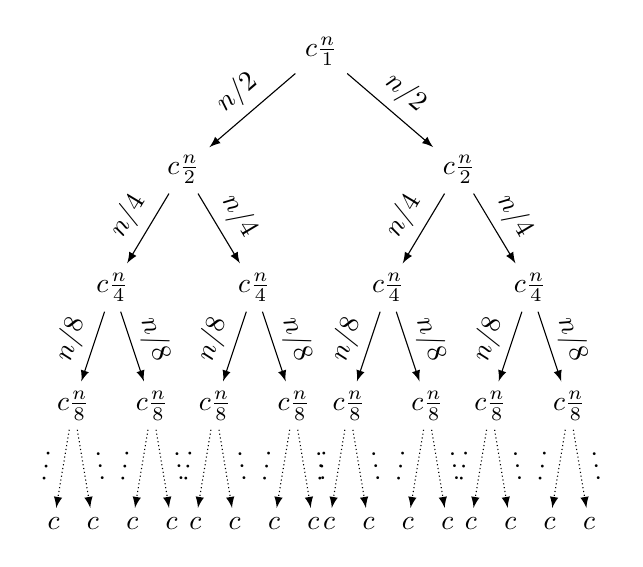
\begin{tikzpicture}[
				level 1/.style={sibling distance=3.5cm, level distance=1.5cm},
				level 2/.style={sibling distance=1.8cm, level distance=1.5cm},
				level 3/.style={sibling distance=1cm, level distance=1.5cm},
				level 4/.style={sibling distance=0.5cm, level distance=1.5cm},
				grow=down,
				edge from parent/.style={draw, -latex, sloped, anchor=south, above},
				edge from parent path={(\tikzparentnode) -- (\tikzchildnode)}
			]
			% Nodo raíz
			\node {$c\frac{n}{1}$}
			% Primer nivel de hijos
			child { node {$c\frac{n}{2}$}
					% Segundo nivel de hijos
					child { node {$c\frac{n}{4}$}
							% Tercer nivel de hijos
							child { node {$c\frac{n}{8}$}
									% Cuarto nivel (hojas)
									child { node {$c$}
											edge from parent[draw, densely dotted] node[auto] {$\cdots$}
										}
									child { node {$c$}
											edge from parent[draw, densely dotted] node[auto] {$\cdots$}
										}
									edge from parent node[auto] {$n/8$}
								}
							child { node {$c\frac{n}{8}$}
									child { node {$c$}
											edge from parent[draw, densely dotted] node[auto] {$\cdots$}
										}
									child { node {$c$}
											edge from parent[draw, densely dotted] node[auto] {$\cdots$}
										}
									edge from parent node[auto] {$n/8$}
								}
							edge from parent node[auto] {$n/4$}
						}
					child { node {$c\frac{n}{4}$}
							child { node {$c\frac{n}{8}$}
									child { node {$c$}
											edge from parent[draw, densely dotted] node[auto] {$\cdots$}
										}
									child { node {$c$}
											edge from parent[draw, densely dotted] node[auto] {$\cdots$}
										}
									edge from parent node[auto] {$n/8$}
								}
							child { node {$c\frac{n}{8}$}
									child { node {$c$}
											edge from parent[draw, densely dotted] node[auto] {$\cdots$}
										}
									child { node {$c$}
											edge from parent[draw, densely dotted] node[auto] {$\cdots$}
										}
									edge from parent node[auto] {$n/8$}
								}
							edge from parent node[auto] {$n/4$}
						}
					edge from parent node[auto] {$n/2$}
				}
			% Segundo hijo del primer nivel
			child { node {$c\frac{n}{2}$}
					child { node {$c\frac{n}{4}$}
							child { node {$c\frac{n}{8}$}
									child { node {$c$}
											edge from parent[draw, densely dotted] node[auto] {$\cdots$}
										}
									child { node {$c$}
											edge from parent[draw, densely dotted] node[auto] {$\cdots$}
										}
									edge from parent node[auto] {$n/8$}
								}
							child { node {$c\frac{n}{8}$}
									child { node {$c$}
											edge from parent[draw, densely dotted] node[auto] {$\cdots$}
										}
									child { node {$c$}
											edge from parent[draw, densely dotted] node[auto] {$\cdots$}
										}
									edge from parent node[auto] {$n/8$}
								}
							edge from parent node[auto] {$n/4$}
						}
					child { node {$c\frac{n}{4}$}
							child { node {$c\frac{n}{8}$}
									child { node {$c$}
											edge from parent[draw, densely dotted] node[auto] {$\cdots$}
										}
									child { node {$c$}
											edge from parent[draw, densely dotted] node[auto] {$\cdots$}
										}
									edge from parent node[auto] {$n/8$}
								}
							child { node {$c\frac{n}{8}$}
									child { node {$c$}
											edge from parent[draw, densely dotted] node[auto] {$\cdots$}
										}
									child { node {$c$}
											edge from parent[draw, densely dotted] node[auto] {$\cdots$}
										}
									edge from parent node[auto] {$n/8$}
								}
							edge from parent node[auto] {$n/4$}
						}
					edge from parent node[auto] {$n/2$}
				};
		\end{tikzpicture}

		\columnbreak

		\begin{enumerate}
			\item Llamado sin coste asociado.
			\item $\to \text{cost}:~2^0c\frac{n}{2^0}$
			\item $\to \text{cost}:~2^1c\frac{n}{2^1}$
			\item $\to \text{cost}:~2^2c\frac{n}{2^2}$
			\item $\to \text{cost}:~2^3c\frac{n}{2^3}$
			\item $\vdots$
			\item $\to \text{cost}:~\log n$
		\end{enumerate}

	\end{multicols}
	El coste $h=cn+cn+\cdots+cn=\lg n$, por $l=\lg n+1$. Hallando su complejidad tenemos:
	$$
		cost:\sum_0^{\lg n+1}cn=cn(\lg n +1)
	$$ $$
		T(n)=cn\lg n+cn=\Theta(n\lg n)
	$$
\end{example}

\subsection{Método del teorema maestro}
Aplicado sobre funciones DyV \textit{(ex: $aT(n/b)+f(n)$)}, donde los problemas generan sub-problemas independientes.
\begin{theorem}[Casos]
	Son mutuamente excluyentes.
	\begin{enumerate}
		\item $f(n)\in O(n^{\lg_b{a-\epsilon}}),
			      \epsilon\in\mathbb{R}^{+}-\{0\}
			      \implies T(n)=\Theta(n^{\lg_ba})$
		\item $f(n)\in \Theta(n^{\lg_ba})
			      \implies T(n)=\Theta(n^{\lg_ba}\lg n)$
		\item $f(n)\in \Omega(n^{\lg_b{a+\epsilon}}),
			      \epsilon\in\mathbb{R}^{+}-\{0\}~si~af(n/b)\le cf(n)
			      \implies T(n)=\Theta(f(n))$, es aquí particular la \textbf{condición de regularidad} \textit{(La función tiene que ser más grande que la función en sus partes o en lo sumo igual)}.\\
		      Las constantes definidas son $b>a\ge1$ y en $1>c>0$.
	\end{enumerate}
\end{theorem}

\begin{example}
	Tiene muchas versiones (veremos el maestro principal), algunos autores dividen las clases (e.g. teorema maestro)
	\\
	Aplicado sobre $msort$:
	Definimos $a\ge2, b>1$.


	Caso 01: Tenemos $cn\in O(n^{\lg_22-0.1})\implies cn \stackrel?= O(n^{0.9})
		\implies cn\ne cn^{0.9}$. Por ende, queda descartado.\\
	Caso 02: Tenemos $cn\in \Theta(n^{\lg_22})\implies cn \stackrel?= \Theta(n\lg n)$. Se cumple, hallamos la complejidad directamente.
\end{example}

\begin{example}
	Trabajaremos con la ecuación de QuickSort en su mejor escenario:
	$$ T(n)=2T(n)+cn $$
	Entonces verificamos que cumpla la forma y $a, b$ funcionan. Pero el hecho que cumpla con la forma no implica siempre de una solución.
	//
	Determinamos $f(n)=cn$ y aplicamos por caso:
	\begin{enumerate}
		\item $Cn\stackrel?=O(n^{\lg_22-\epsilon})$
		      En estas polinomiales el exponente es fundamental
		      Si tenemos que $\epsilon=0.0\cdots01$. Como notamos esta función no satisface puesto

		\item Notamos que acá si se cumple, podemos sacar el límite y esto debe darnos una constante (no 1).
	\end{enumerate}
	Vemos que nos dió el orden, no la función de eficiencia. Lo que nos interesa siempre, eventualmente es el orden.

\end{example}


\subsection{Método de la sustitución inteligente}
Consiste de los pasos:
\begin{enumerate}
	\item Suponer solución.
	\item Demostrar con PIM que es funcional (hallar ctes).
\end{enumerate}

\begin{example}[Similar a msort]

	Se tiene la función $T(n)=2T\floor{n/2}+n$\\
	Notamos como $msort=2T(n/2)+cn\land T(n)\in O(n\lg n)$\\
	Suponemos $k=\frac n2$, por lo que $k<n$.\\
	Sustituímos en la ecuación de recurrencia:
	$$ T(n)\le 2(c\floor{n/2}\lg \floor{n/2})+n $$
	$$ \le cn\lg \floor{n/2}+n$$
	$$ \le cn\lg \floor n-cn+n$$
	$$ \le cn\lg n;\quad c\ge1$$

	Debemos mostrar solución cumple: Condición límite $\land$ Casos base.

	Notamos como no cumple $n=1$ puesto
	$$ T(1)\le c~1\log 1 $$
	No obstante cumple para constantes superiores.
	$$ T(2)\le c~2\lg 2 $$$$
		T(2)\le c~3\lg 3 $$
	Tomando ventaja de la Notación asintótica, reemplazamos casos base ($c.b.$) en la prueba inductiva.
	$$ T(n)=2T\floor{n/2}+n $$$$
		\therefore T(2)=2(1)+2=4 $$$$
		\therefore T(3)=2(1)+3=5
	$$
	La prueba inductiva dicta $T(n)\le cn\lg n$ y un $c\ge2$, tenemos:
	$$
		T(2)\le c~2\lg 2    $$ $$
		T(3)\le c~3\lg 3
	$$
	Es importante considerar que la \textbf{prueba inductiva $\ne$ ec. recurrencia}.
\end{example}



\subsection{Método de ecuación característica}
Es aplicado sobre ecuaciones de recurrencia lineales homogeneas (ER-LH) de la forma
$$ a_0T(n)=a_1T(n-1)\pm\cdots\pm a_kT(n-k) $$
$$ x^n=T(n);\quad T_0=I_0;\quad T_1=I_1;\quad\cdots;\quad T_{k-1}=I_{k-1}.$$
\begin{definition}[Ecuación característica]
	$$a_nT_n+a_{n-1}+T_{n-1}+\cdots+a_{n-k}T_{n-k}=0$$
	$$ =a_nT_k+a_{n-1}T_{k-1}+\cdots+a_kT_0=0 $$
	$$ \implies a_0x^k+a_1x^{k-1}+\cdots+a_kx^0=1 $$
	Con raíces $r:r_1,r_2,\cdots,r_k$.
	Sean distintas y de multiplicidad 1 ó múltiples de multiplicidad.
	\begin{theorem}[Mult. = 1]
		$$T(n)=\sum_{i=1}^n c_ir_i^n$$
	\end{theorem}
\end{definition}

\begin{example}[Sobre Fibonacci]
	Defínase $T(n)=T(n-1)+T(n-2);~ T(0)=0;~ T(1)=1.~ n\in\mathbb{Z}^+$.\\
	Primero obtenemos la ecuación característica:
	$$ 1T(n)-1T(n-1)-1T(n-2)=0;\quad T(n-k)=x^{n-k} $$
	$$ 1x^{2-0}-1x^{2-1}-1x^{2-2}=0 $$
	$$ x^2-x-1=0 $$
	Mediante la cuadrática hallamos las raíces, son $r_{1,2}=\frac12(1\pm\sqrt5)$. Notamos que son distintas, aplicamos el teorema para mult. = 1.
	$$ T(n)=c_1[\frac12(1+\sqrt5)]^n+c_2[\frac12(1-\sqrt5)]^n $$
	Aplicado sobre los casos base T(0) y T(1):
	$$ T(0)=c_1[\frac12(1+\sqrt5)]^0+c_2[\frac12(1-\sqrt5)]^0 $$
	$$ T(1)=c_1[\frac12(1+\sqrt5)]^1+c_2[\frac12(1-\sqrt5)]^1 $$
	Resta resolver el sistema $2\times2$ y entonces obtendremos la complejidad del algoritmo.
\end{example}